% 
% Annual Cognitive Science Conference
% LaTeX Paper -- Proceedings Format
% 

% Original : Jin-Hwa Kim (jhkim@bi.snu.ac.kr)        06/02/2014
% Modified : Jin-Hwa Kim (jhkim@bi.snu.ac.kr)        06/22/2014

%% Change ``a4paper'' in the following line to ``letterpaper'' if you are
%% producing a letter-format document.

\documentclass[10pt,letterpaper]{article}
\usepackage{cogsci}
\usepackage{pslatex}
\usepackage{apacite}
\usepackage{graphicx}

\title{Active Long Fixation Correlates with the Formation \\
  of Long-Term Memory and Its Computational Modeling}
 
\author{{\large \bf Jin-Hwa Kim (jhkim@bi.snu.ac.kr)} \\
  Cognitive Science Program, Seoul National University \\
  Seoul, 151-742, Republic of Korea
  \AND {\large \bf Byoung-Tak Zhang (btzhang@bi.snu.ac.kr)} \\
  School of Computer Science and Engineering, Seoul National University \\
  Seoul, 151-742, Republic of Korea}

\begin{document}

\maketitle

\begin{abstract}
Enhanced prospects for the application of eyewear demands the study on the eye movements beyond the reading task. We investigated the eye movements of the subjects watching the kids video. The characteristics of the eye movements are analyzed by the observation of the marginal distribution of fixation durations. The marginal distribution of fixation durations for the video stimuli has a different shape to that for the reading task. The video stimuli causes the fast-falling period for the shortest fixation durations unlike to the slow-rising ones for reading, and the fixation durations that are longer than two seconds show the increasingly fluctuated frequencies. The former beacuse of the relatively undemanding load for the cognitive process and the continuous change of given stimuli; the latter because of the spatio-temporal constraints of given stimuli. We classified the constraints generating the long fixations into three types. However, we found that, among the constraints, the long fixations which are voluntarily engaged associate with long-term memory than any other types. Finally, we propose the computational modeling to predict those active long fixations, which may provide the way to effectively summarize the story of a given video.

\textbf{Keywords:} 
Eye movement; fixation; spatio-temporal; long-term memory, computational modeling.
\end{abstract}


\section{Introduction}

The brain is the most intelligent organ of the human body. It receives many different forms of the sensory information and processes these information appropriately with regard to its nature for doing well. Especially, the visual information takes a very special position among other kinds of sensory information as it does not need to touch or smell it directly, causing the chemical reaction inside the body, and is transfered to the remote target far freely than any other types of the sense. Furthermore it gives more chance to survive in the situation of being threaten by the predators using the eyes to detect the foes in the remote place before their approaching. 

But this notable advantage is not freely given one as it requires more delicate and clever way of interpreting the visual information. Because the visual information can easily be affected by the moment-to-moment environmental changes, heuristic but robust compensation strategies are demanded. So, how the brain processes the visual information provides the profound way to study the mechanism that the brain precisely and efficiently processes the most dynamic and enormous sensory information.

There are a lot of studies on the computational modelling for the visual information, which include the visual fragment completion, the scene or object classification and recognition \cite{winn2005,lazebnik2006}, and object tracking \cite{YiWu2013}. These research topics often tend to focus on the objective for each tasks, not on the implementation of the method how the brain deals with. As a result, the computational approach to the modeling for the visual information processing of the brain is gradually changed to the optimization problem to effectively solve, which hinders the understanding of the human-level information processing abilities. 

Particularly, the object tracking seems to describe how we keep the attention toward the interesting object, however, the eye movement, which is mostly controlled by the oculomotor system, is better to imply the way of how the brain works for the acquisition of the visual information \cite{Henderson2003}. For an instance, in the fixation state the human eyes only recognize the small portion of the whole sight. If you read this paper in a 8-inch distance fixing on one particular letter, you cannot read next two words or approximately about ten letters which are presented in the para-fovea. For the brain is well-known for its parallel processing on the neural circuits, this sequential notion of eye movement visual system does not suit to the efficiency of the brain.

In comparison with the reading eye movement, which are relatively well studied by psychologists and neuroscientists \cite{Rayner1998,Reichle1998}, the study of the eye movement on the video stimuli has been neglected or avoided due to the uncertainty of the research theme or its application \cite{Tatler2011}. However, the recent advancement of the sensory device, like the Google Glass and the mobile devices for the eye tracking, enables to study on the more natural experimental environment and to implement the research model or applications on those mobile device. Moreover, there is a different aspect of studying on the eye movement for video stimuli. How long the fixation sustains is more constrained by the video content rather than the reading materials do, and the selection of the next fixation and the saccadic movement direction tend to be more liberal than the dominance of horizontal searching of reading does. 

In this study, we investigate the characteristics of eye movements toward the video stimuli. The basic elements of the eye movements can be segregated into the fixation duration and the saccade vector, which consists of the saccade direction and the length of the saccadic movement \cite{Findlay1999,Feng2006}. In this study, we focus on the characteristics of the fixation duration as the evidence of the cognitive process.

\section{Materials and Methods}

\subsection{Experiment 1}

For this study, we prepared the video meterial \textit{Pororo Season 3}, which is a famous kids video in Republic of Korea. In this video, there are simple shaped artificial 3D-rendered characters which have marked individualities. \textit{Pororo Season 3} contains the 13 consecutive episodes that each episode has a single storyline. Remarkably, 4 characters are intervene to the main plot among the existing characters, the cybertic aliens \textit{Popo} and \textit{Pipi} in the first episode, the homemade robot \textit{Rody} in the episode 3 and the magician Tongtong in the episode 6. Though the experiments and the analyses using these features are not fully considered in this study, we look forward to publish the results soon. 

We recruit 17 participants with normal vison (11 males, 6 females; 23-31 years of age; median is 25), who are voluntarily participate in the study. All participants had not experienced a brain damage or a behavioral disorder. The participants are new to the video, \textit{Pororo Season 3}. Experimental procedures were agreed by the Research Ethics of Seoul National University and the participants signed a consent form.

Participants watched the kids video in the room which has the experimental setttings. The room is about 3 square meters surrounding by the opaque curtains. On the side of the room, an widescreen HDTV (1920x1080 resolution, 885cm x 500cm, 16:9 ratio) is installed, and 2.1 channel speakers. Participants are guided to sit down on the comfortable sofa in front of 1.7m from TV screen.

Eye movements and concurrently the user-perspective scenes are recorded by \textit{Tobii Glasses eye tracker}, the corneal reflection based system with a sampling rate of 30 Hz. We used the \textit{I-VT algorithm} as the fixation filter (system default), which classifies the fixations with the velocity threshold, 30 degree per second. Usually, the saccadic eye movements are discriminated between low velocities (less than 100 degree/second) and high velocities (higher than 300 degree/second), velocity-based classification is simple but reasonable \cite{Salvucci2000}.

We classified the event type of the eye movements into three categories; fixations, saccades and unclassified. The unclassified data is discarded and not used in this study.

\begin{figure}
  \centerline{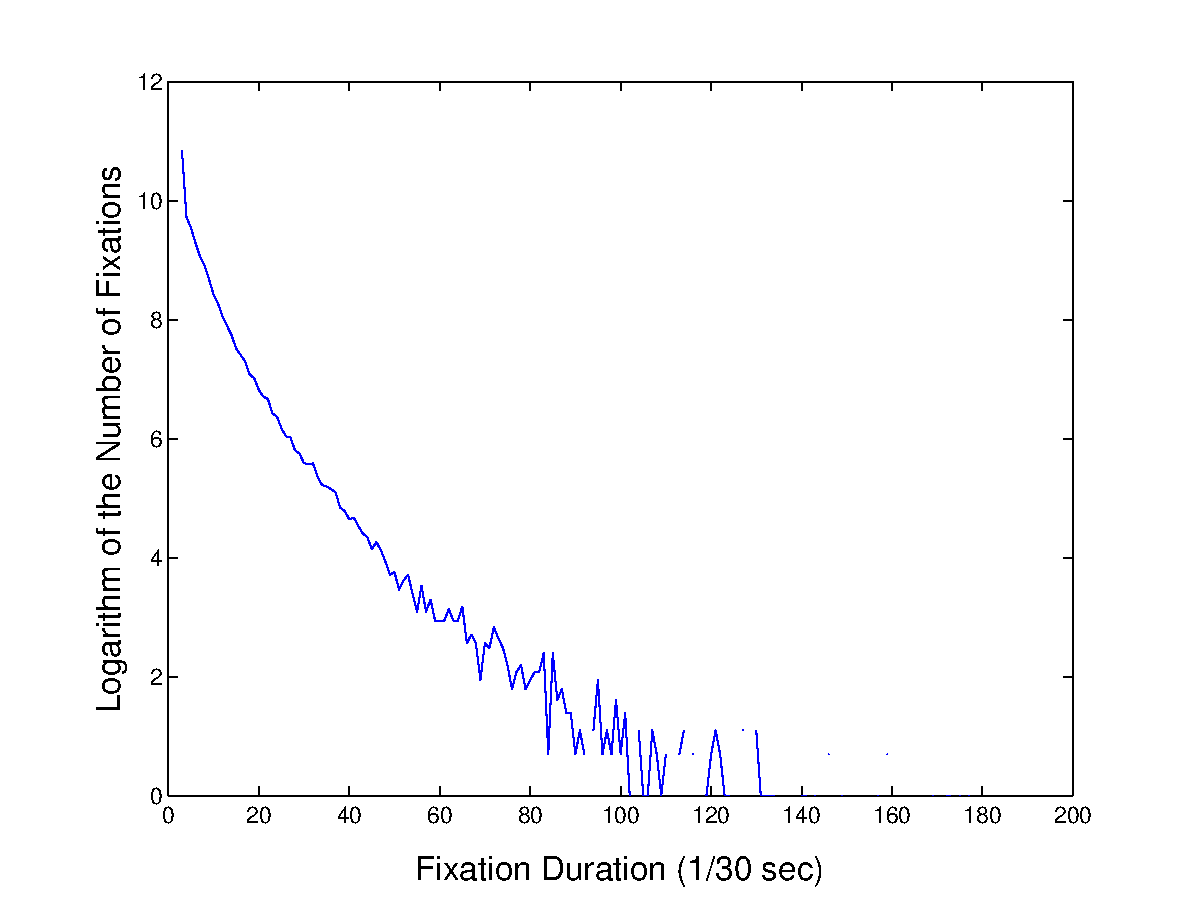
\includegraphics[width=86mm,trim=10mm 3mm 10mm 3mm]{./eps/marginal_fixation_duration.eps}}
  \caption{Marginal distribution of fixation duration. All of the 147,974 fixation information of 17 participants is used. The X-axis represents the number of time unit, 1/30 sec., therefore, 30 indicates 1 second. The Y-axis represents the logarithm of the number of fixation durations which are the same time length with regard to the time unit of X-axis. Fixation durations which are longer than about 2 seconds are getting more unpredictable along with increasing the fixation duration.}
  \label{fig:marginal-fixation-duration}
\end{figure}

\subsection{Experiment 2}

For 12 participants who have participated in \textit{Experiment 1}, we prepared the controlled memory test for each participant. We conduct this experiment 3-4 months later after \textit{Experiment 1} (the intervals are not consistent due to a schedule conflict). A memory test consists of total 20 video sequences; 8 sequences for long fixations, another 8 sequences for short fixations, and the remaining 4 sequences for the controll, which are not seen in the previous experiment. The lengths of all video sequences are the same as 3 seconds. \textit{The long fixation sequences} are randomly picked from each participant's data containing the longer than 2 seconds of fixation in the middle of the sequence. \textit{The short fixation sequences} are randomly picked from each participant's data containing the shorter than 300 milisecond. The 4 control sequences are randomly picked from the other season of \textit{Pororo} series, \textit{Pororo Season 2}.

Each participant identifies 20 sequences randomly sorted. Each participant gives a sequence 1 to 5 score depending on the assurance of whether he or she saw the sequence before or not. 

\section{Fixation Duration}

Fixation duration shows the characteristic of the eye movement patterns on the visual stimuli. As our expectation, fixation duration change substantially up to 10 seconds during watching the video. These changes are partly caused by the sequential changes of the visual stimuli, the fluctuated responses of the oculomotor system and cognitive processes. As the length of fixation duration is not a deterministic property, because more than a single system dynamically contribute to the final motor command for the oculomotor system, we assumed the fixation duration as the random variable with probabilistic distribution \cite{Rayner1998,Reichle2004,Reichle2006}.

\subsection{Marginal Distribution of Fixation Durations}

Figure~\ref{fig:marginal-fixation-duration} shows the marginal distribution of fixation duration, which includes all of the 147,974 fixation durations of 17 participants. The X-axis represents the duration time, and the Y-axis represents the log scale of the number of fixation durations across the whole data. For further details, refer to the caption of Figure~\ref{fig:marginal-fixation-duration}.

The shape of the marginal distribution of fixation duration (Figure~\ref{fig:marginal-fixation-duration}) is illustrated with the exponential function (see the logarithm of the Y-axis). While the distribution of the \textit{reading} fixation durations has a quiet different shape \cite{Feng2006}. The shape is roughly segmented into three parts, slow-rising ones for short fixations, fast-rising period until around 180 ms, and following a long tail for long fixation durations. These facts allow us to think that 180 ms of the fixation duration for reading is the most general case, but obviously not for watching the video.

Fixation durations which are longer than about 2 seconds are getting more unpredictable along with increasing the fixation duration. The content of the video stimuli might has the responsibility to these effects. The fixations more tend to maintain the gaze position when the visual constraint imposes. Surprisingly, the visual constraints have more various form than we expected.

\begin{figure*}
  \centerline{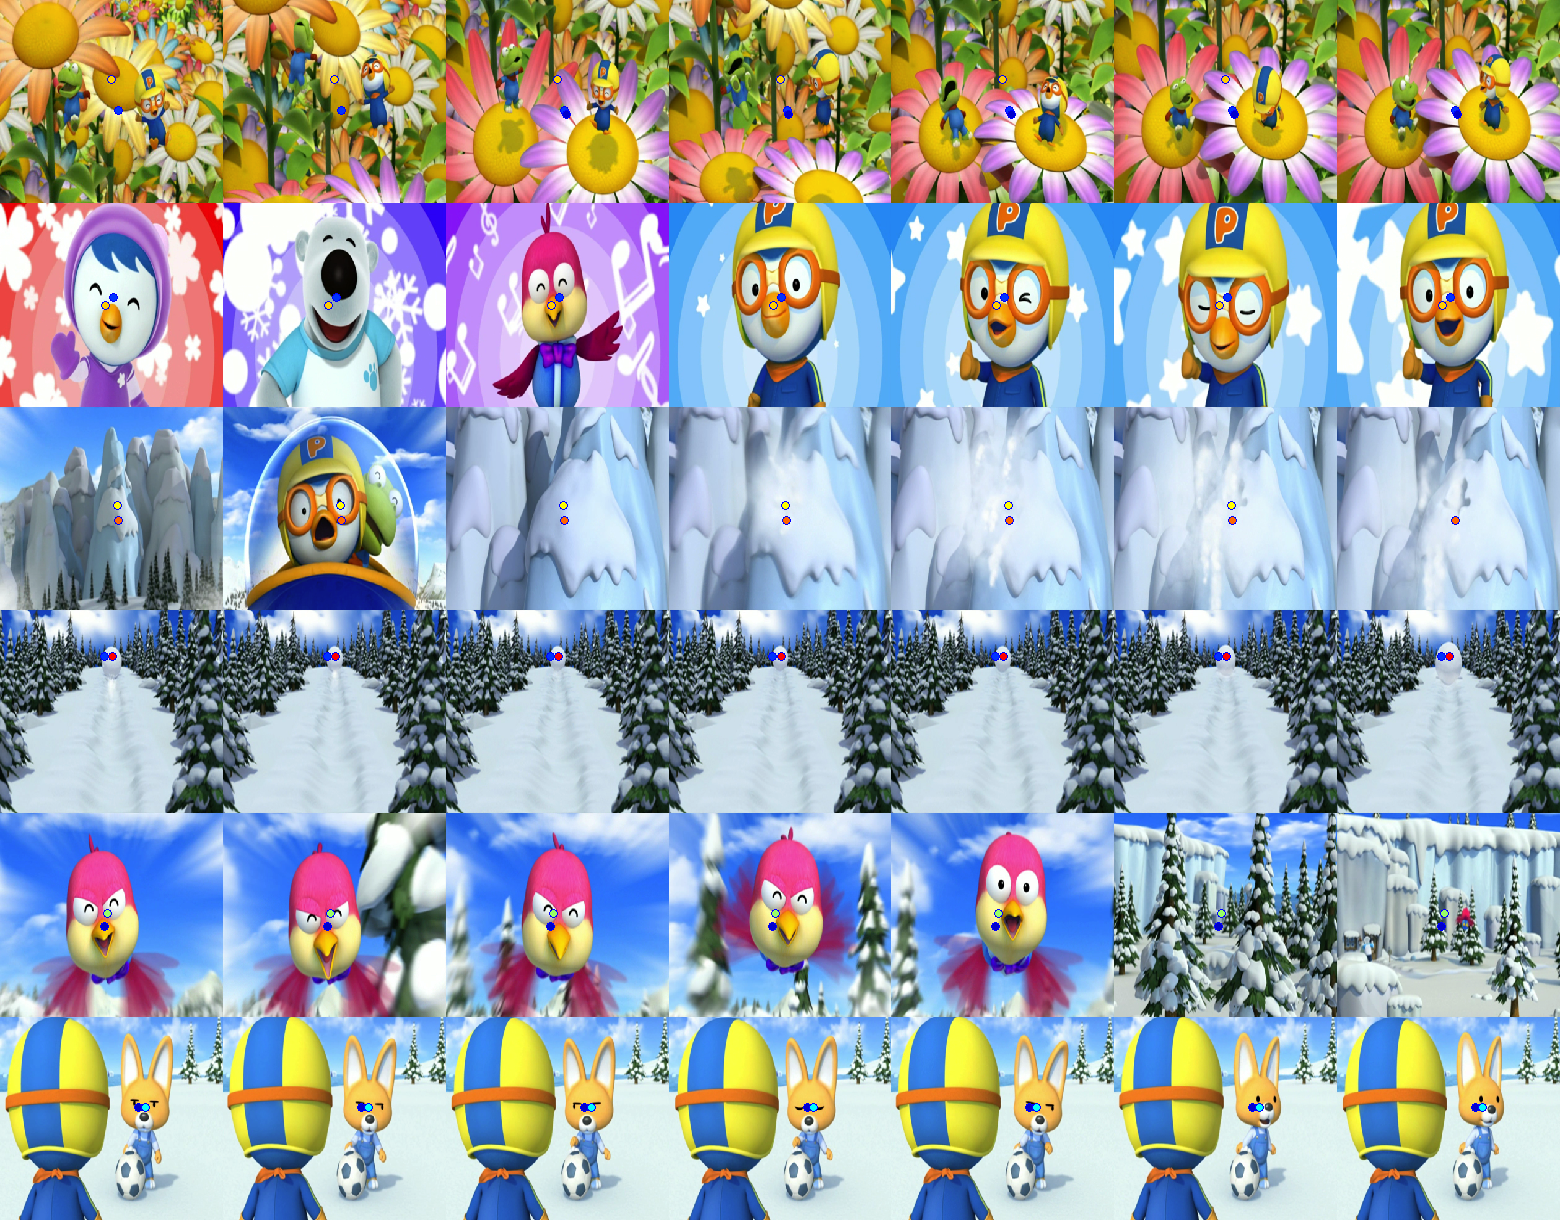
\includegraphics[width=178mm]{./eps/long_fixations.png}}
  \caption{The sequences of frames which receive more than 3 seconds of the fixation duration from the participants. We piled up the number of the fixations which are longer than 3 seconds. And We set the threshold as equal or larger than 12 and we got 11 sequences across 1 hour 7 minutes 50 seconds length of the material. We randomly chose 6 out of 12 sequences for the review. Each row means the independent sequence and each column means the single frame. The time interval between the frames is 500 ms. The colored dots mean the fixation, which are longer than 3 seconds. The same color means the same participant. The first row of the sequence shows that \textit{Pororo} and \textit{Crong} just jumped out of the shoulder of \textit{Tongtong} who was flying in the sky. Two sunflowers spring \textit{Pororo} and \textit{Crong} into the sky in multiple times. But due to the perspective of the camera, the location of the two characters in the scene is almost fixed. Participants fixated their eye gaze on the middle of two characters while the background shifting up and down.}
  \label{fig:long-fixations}
\end{figure*}

\begin{table*}[!ht]
\begin{center} 
\caption{Long Fixation Types.} 
\label{long-fixation-types} 
\vskip 0.12in
\begin{tabular}{ll} 
\hline
Long fixation type    &  Description \\
\hline
Contrast Focus        &   The background is rapidly changing while the object 
                          is staionary. \\
Alert Focus           &   An urgent situation happens with an object, which can 
                          be easily targeted as a cause. \\
Successive Focus      &   Successive changes to keep attracting. \\
\hline
\end{tabular} 
\end{center} 
\end{table*}

\subsection{Long Fixation Durations}

In Figure~\ref{fig:long-fixations} the sequences of frames which receive more than 3 seconds of the fixation duration from the participants are shown. We piled up the number of the fixations which are longer than 3 seconds on each 200 ms time window. Each time window can have up to 102, because, in 200 ms, six data points are available for our experimental condition (30 Hz sampling rate), and those data points are generated from the independent multiple sources of 17 participants. We set the threshold as equal or larger than 12, which means at least two different participants should be involved in. We got 11 sequences across 1 hour 7 minutes 50 seconds length of the material. We randomly chose 6 sequences for the review. Each row means the independent sequence and each column means the single frame. The time interval between the frames is 0.5 seconds. The colored dots mean the fixation, which are longer than 3 seconds. The same color means the same participant. The interval times of the sequences are, from the first row to the last one, 26.4s to 29.6s; 1m 25.4s to 1m 28.4s; 3m 50.8s to 3m 53.6s; 15m 27.4s to 15m 30.6s; 34m 13.0s to 34m 16.2s; and 53m 8.0s to 53m 11.0s.

The first row of the sequence shows that \textit{Pororo} and \textit{Crong} just jumped out of the shoulder of the magician dragon \textit{Tongtong} who was flying in the sky. Two sunflowers spring \textit{Pororo} and \textit{Crong} into the sky in multiple times. But due to the perspective of the camera, the location of the two characters in the scene is almost fixed. Participants fixated their eye gaze on the middle of two characters while the background shifting up and down. The third row of the sequence is the scene that the airplane crushed into the mountain. Snowflakes are blown off from the point of the impact.

Figure~\ref{fig:long-fixations} shows that the long fixation durations appear when the location of the characters in the scene is relatively fixed and the background is drastically shifted up and down (first), the close up characters are serially shown up in the middle of the screen (second), a tense situation that the \textit{Pororo}'s airplane clashed with the snowy mountain, which was seen in the middle of the scene (third), an urgent moment that a huge snowball is about to roll down back the hill, which was previously rolled up by the robot \textit{Rody} (fourth), the enchanted mighty \textit{Harry} flies very fast, so the background is blurred (fifth), and \textit{Eddy} rolled his eyes to kick his ball avoiding the opponent \textit{Pororo} (last). These long gazed sequences can be categorized into three types. The first type is the \textit{Contrast Focus}, when the background is rapidly changing while the character (the featured object) is fixed on the screen (refer to the first and fifth). The second type is the \textit{Alert Focus}, when an urgent situation happens with an object which can be easily targeted as a source of the trouble (the third, fourth and sixth). The last type is the \textit{Successive Focus}, appearing a single object in the middle of the screen, and then successively changing the object to another one constantly attracting the audience's attention (the second). Table~\ref{long-fixation-types} recaps the long fixation types.

These various types of the long gazed sequences show that a naive approach to the predict the visual constraint which induces the long fixation using a single analytical method, like the salient feature detectors \cite{marr1980,canny1986} or the optic flow \cite{koenderink1986} would fail. The \textit{Contrast Focus} and \textit{Successive Focus} types can be estimated by using the combination of the appropriate feature detectors and the optic flow, and the temporal modeling of the attention. However, the \textit{Alert Focus} cannot be solved without the cognitive modeling for the scene comprehension, which is related to the emotion-based reaction. The proposal of the solution is beyond the scope of this study, though it is the worthwhile issue (see Discussions).


\section{Discussions}

The marginal distribution of the fixation duration shows the characteristics of the response toward the visual stimuli. The shape of the marginal distribution of fixation duration can be estimated as the exponential function though the marginal distribution of the reading fixation durations is illustrated as a left-skewed normal distribution, peaking at 180 ms. Then why reading and watching are so different from each other in this property? The first to think is the difference of the cognitive process during the fixation. Simply put, reading involves the visual processing in addition to the lexical processing. The visual process captures the letters through the retina, Lateral Geniculate Nucleus (LGN) and the primary visual cortex. Then the information of the letters is directed to the distributed lexical processing areas. Though skipping is occasionally occurred while reading, those serial processes spend some latency time. Since reading is an active task, the subject decides when and where to move to a next word, those latencies tend to be preserved. By the way, watching the video has a different condition. The lexical processes are typically not needed, which are heavy tasks in time. Also the video stimuli are passive in regard to the temporal aspect. Therefore the generation of the long fixation duration is sufficiently constrained by the duration of the stimulus, at the same time, the content of the stimulus. 

We recap the visual constraints which trigger the long fixation durations as three types in Table~\ref{long-fixation-types}. The \textit{Contrast Focus} type seems that the contrast effect attracts the attention and marks the featured object. The second type, \textit{Alert Focus}, is an ongoing urgent situation that makes the eyes fixates an object which is thought to be a cause or a factor. The last type is the \textit{Successive Focus}. It looks like the successive appearing of the objects keeps the fixation longer, however, the interpretation that the successive absence of the other attracting elements just let the fixation persist is also possible. After all, what is the meaning of the long fixation durations on the video stimuli? Despite of the fact that it could be a latency time to process the cognitive information of the visual stimuli, in the other perspective, it is an waiting time to the potential salient moment on that eye position. All participants are grown-up persons, so familiar with almost all kinds of events in the episode of the video. Easily predicted, and waiting on the prospective location for a dramatic change or a new event is practical.

The computational modeling of the long fixation durations is worth to discuss. As we discussed, the long fixations are constrained by the visual content of the video stimuli, the probabilistic modeling of that would be unsuccessful to compatible with the unprecedented stimuli. The first possible attempt is the composition of the salient detectors \cite{marr1980,canny1986} and the optic flow \cite{koenderink1986} accompanying the tentative cognitive modeling of that. As there are the types of the long fixation durations, the cognitive modeling can be projected to the lower dimension of the search space. Additionally, the estimation of the eye tracking is viable on top of the model. The serial information of the fixation positions enables us to intelligently select the portion of the visual features on the scene, like a human, it can be a breakthrough for the cognitive modeling on the endless stream of the visual information.


\section{Conclusions}

We studied the characteristics of the eye movements through the marginal distribution of fixation durations. We notice that the marginal distribution of fixation durations for the video stimuli has a form which is different from the marginal distribution of fixation durations for the reading materials. The behavioral basis for the difference may attribute to the lighter load for the cognitive process and the temporal and spatial constraints which are given by the video stimuli. Those constraints are summed up as three distinctive types, Contrast Focus, Alert Focus and Successive Focus. Also, we present the tentative suggestion for the computational modeling of the eye movements using the combination of the feature detectors and the optic flow in aid of the cognitive modeling.


\section{Acknowledgments}

This work was supported by the National Research Foundation of Korea (NRF) grant funded by the Korea government (MSIP) (NRF-2010-0017734-Videome), supported in part by KEIT grant funded by the Korea government (MKE) (KEIT-10035348-mLife, KEIT-10044009).

\bibliographystyle{apacite}

\setlength{\bibleftmargin}{.125in}
\setlength{\bibindent}{-\bibleftmargin}

\bibliography{eye_tracking}

\end{document}
